% Allow relative paths in included subfiles that are compiled separately
% See https://tex.stackexchange.com/questions/153312/

\providecommand{\main}{..}
\newcommand{\decfirst}{\textit{Decision.1}}
\newcommand{\decsecond}{\textit{Decision.2}}
\documentclass[\main/thesis.tex]{subfiles}

\externaldocument{}


\begin{document}
\chapter{Making Noise, Hearing Drums}
\label{implementation}


\section{What Are We Doing Again?}
Our goal is to create a system for the generation of novel drum sounds. So far, we've discussed what tools to pick for virtual synthesis, and how to represent digital sounds in a smaller, more \enquote{learn-able} format. In this chapter, we will discuss the two main components of  system: The \textit{virtual synthesizer} and the \textit{virtual ear}.

A visual representation of this pipeline is given in  Figure~\ref{fig:pipeline_outline}. In Section~\ref{vs}, we discuss the implementation of a virtual synthesizer which can create a wide variety of noise. In section~\ref{sec:ear}, the implementation of the virtual ear is discussed.


\section{Virtual Synthesizer}
\label{vs}
 \begin{figure}[h!]
    \begin{center}
    \textbf{Pipeline Design}
    \makebox[\textwidth]{
    \fbox{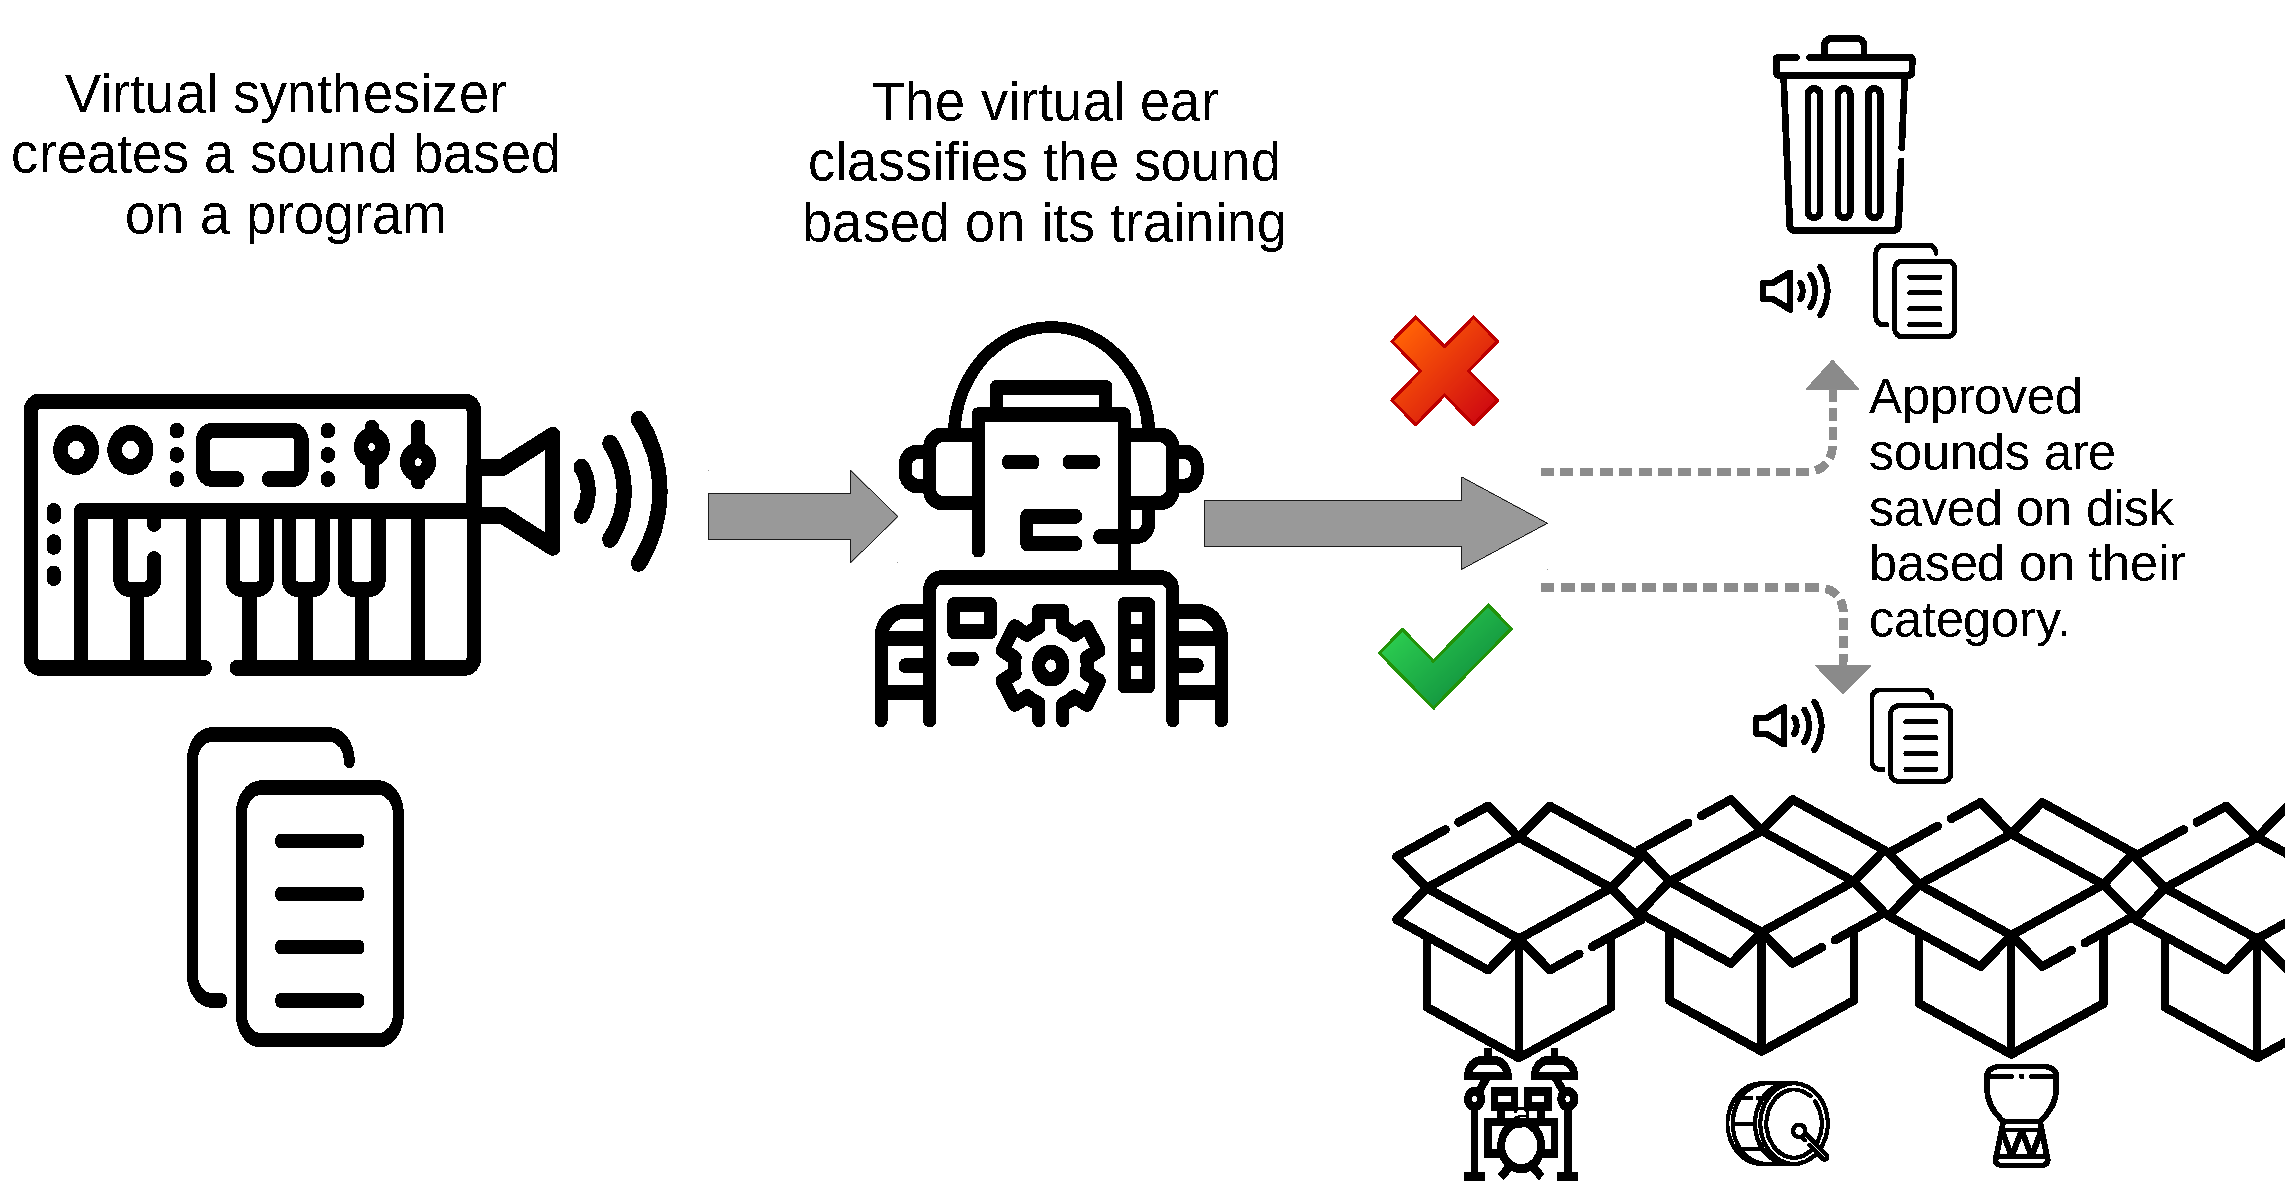
\includegraphics[width=1.1\linewidth]{images/chapter_4/pipeline.pdf}}}
    \end{center}
    \caption{An implementation which allows for easy parallelization when needed. Virtual synthesizer rapidly generates random programs and the corresponding sounds, while the virtual ear will listen to the sounds and determine if they should be categorized as drums and if so, which category of drum do they belong to. 
    }
\label{fig:pipeline_outline}
\end{figure}
\subsection{Why DSP over ANN Synthesizers?}
 Rather than using neural networks for sound synthesis, we generate programs for a virtual synthesizer which mainly utilizes additive and subtractive techniques. Our decision is based on the following factors:
\begin{enumerate}[label=(\roman*)]
    \item \textit{Novelty and Creativity}: The goal here is to work with the limitations of any tractable sound source to create its approximations of a given sound category. We seek to create novel sounds via artificial, exploratory creativity. Boden defines this concept as an emergent property of generative work within confined rule sets~\cite{boden2009computer}. An example is the perpetual popularity of 8-bit aesthetics~\cite{collins2007loop}. 
    \item \textit{Interpretability}: Neural networks are often described as black boxes with uninterruptible weights~\cite{basheer2000artificial}. Their highly recursive structure makes modern explanation methods such as saliency maps unreliable~\cite{rudin2019stop}.  
    \item \textit{Speed of Rendering}: Neural network synthesis is costly. Sub 24 khz sample rates are common in most relevant works~\cite{yamamoto2020parallel,oord2017parallel,aouameur2019neural,ramires2020neural}. This is far below CD quality sampling rates~\cite{reiss2016meta}. At our fixed sampling rate of 48 khz, synthesizers with 8 submodules can create and save 1 second sounds to hard-disk with an average rendering time of 50 milliseconds\footnote{Using a single process on a Macbook Air 2012 and Ubuntu 18.04}. 
    \item \textit{Flexibility and Scaling}: Probabilistic audio generation is often done sequentially. State of the art, parallel wave generation with GANs requires a fixed amount of rendering time for each time-step~\cite{yamamoto2020parallel}. With our virtual synthesizer, the added footprint of increasing the length of rendered sounds or higher sampling rates is relatively minuscule.  
\end{enumerate}

\subsection{Virtual Synthesizer Implementation}
 To create sounds, we make use of digital synthesizers capable of rapidly receiving or creating programs, as well as rendering the corresponding sound offline. Classical DSP allows for quick, offline, and parallel generation of audio signals without the usage of GPUs. Pippi\footnote{https://github.com/luvsound/pippi} and SciPy~\cite{jones2001scipy} libraries were extensively used for their DSP functionalities. The virtual synthesizer contains a set of one or more submodules.

 \begin{figure}[htbp]
    \begin{center}
    % \textbf{Synthesizer SubModule }
    \makebox[\textwidth]{
    \fbox{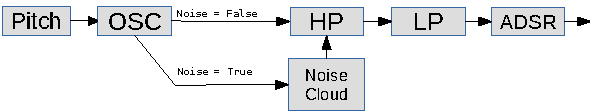
\includegraphics[width=1\linewidth]{images/chapter_3/synthesizer_block.pdf}}}
    \end{center}
    \caption{High level representation of pre-rendering steps for each submodule. Each Synthesizer contains 1 or more submodules. Synthesizer programs set the number of these submodules and their parameters.
    }
\label{fig:submodule}
\end{figure}

 \begin{figure}[htbp]
    \begin{center}
    % \textbf{Synthesizer SubModule }
    \makebox[\textwidth]{
    \fbox{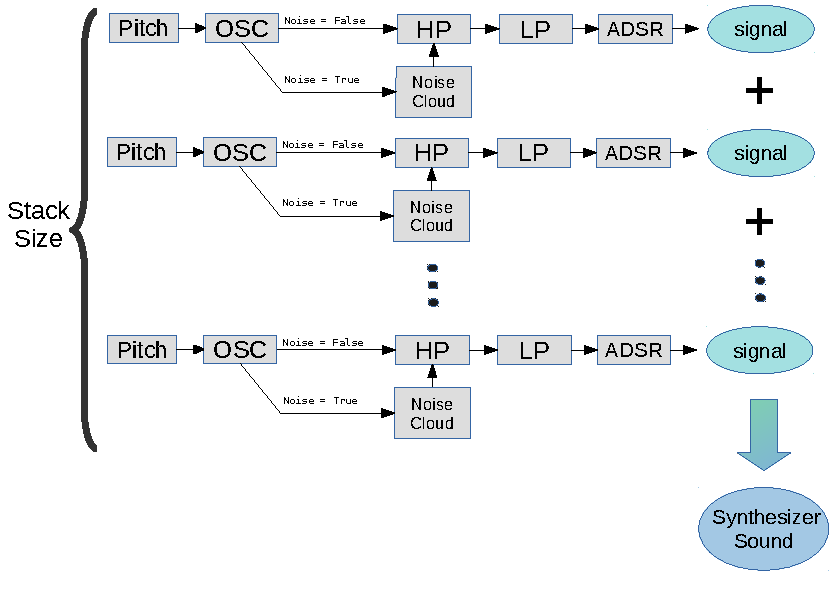
\includegraphics[width=1\linewidth]{images/chapter_3/synthesizer_all_blocks.pdf}}}
    \end{center}
    \caption{The output of the virtual synthesizer is the normalized addition of the output of its submodules. A synthesizer can have any number of submodules. 
    }
\label{fig:synth_modules}
\end{figure}
 Each submodule is a self-contained noise making unit. Submodules have identical sets of parameters, but widely different outputs can be achieved depending on the values assigned to these parameters. The output of the virtual synthesizer is the normalized addition of the output of its submodules. The synthesizer can have any number of submodules. The parameters that dictate the output signal of each submodule as well as the range of values each parameter can take are shown in Table~\ref{table:submodule_params}. We call the number of submodules in each virtual synthesizer the \textit{stack size}. We call the sets of parameter values that characterize a synthesizer's submodules a \textit{program} (analogous to a preset for a VST).  

Since we are interested in short, one-shot percussive sounds, each virtual synthesizer program will generate a 1 second piece of audio. This 1 second limit is over twice the length of the average one-shot drum sample in MixedDB (around 0.4 seconds). Each submodule can make an audio signal with the length of 0.1-1 second, and play it at any point within the 1 second rendering time\footnote{The entire sound must fit within the second, for example, a 0.3 second sound cannot begin playing past 0.7 seconds into the rendering time frame}. If the synthesizer has a stack size of more than 1, the audio signals from each submodule are overlapped and the total amplitude is normalized.

\begin{table}[t!]
\centering
\resizebox{\columnwidth}{!}{\begin{tabular}{ |c|c|c| } 
\hline
Parameters & Value Range & notes and constraints\\
\hline \hline
Attack & 0-3 & A-D-S-R values relative\\
Decay & 0-3 & relative to A-S-R\\
Sustain & 0-3 & relative to A-D-R\\
Release & 0-3 & relative to A-D-S\\
OSC type & sine,square,saw & tone type\\
IsNoise & boolean & whether to \newline use OSC type to generate noise\\
Length & 0-1 second & - \\
StartTime & 0-1 second & Length+Start$<$1\\
Amplitude & 0.1-1 & 1 = max amplitude\\
Pitches(notes) & list of pitches &  range of C0(16.35hz) to B9 \\
HP filter Cutoff & 0-20000hz & -\\
LP filter Cutoff & 20000-HP & never lower than HP cutoff\\
Filter Order & 4,8,16 & butterworth filter order \\
\hline
\end{tabular}}
\caption{Synthesizer submodule parameters. Despite the simplicity of the parameters and efforts at constraining the ranges, the number of parameters that can be randomly chosen for each submodule is in the order of $10^{15}$ }
\label{table:submodule_params}
\end{table}
The ADSR parameters shape the entire amplitude of the signal. Each submodule creates its signal at full amplitude then shapes it according to its internal ADSR parameter. Prior to being applied to the signal, each of these parameters is assigned an integer value in the range of 0-3, and normalized relative to the others such that \[ A_{norm} + D_{norm} + S_{norm} + R_{norm} = 1 \] \\ 
Where each value $v_{norm}$ in the $\{A_{norm}, D_{norm},S_{norm},R_{norm}\} $ set is normalized such that:
\begin{align*}
\text{for each $v$ $\epsilon$ \{A,D,S,R\}} \\
v_{norm} = \dfrac{v}{A + D + S + R}
\end{align*}
 The OSC type will determine the wave-shape of the signal. This parameter is limited to three fundamental wave forms: sine waves, square waves and saw waves. We also allow the creation of noise signals, which can imitate timbral characteristics of higher pitched drum samples at a very low computation cost (relative to the addition of thousands of sine waves at various frequencies). If the IsNoise boolean is set to true, the OSC type parameter loses importance as the wave type will be routed through a noise-cloud. 

Each submodule is a monophonic synthesizer. That is, each submodule can play one note (or frequency) at a time. However, quick changes in pitch can occur in drum sound.  To mimic such sounds, synthesizer submodules may slide between 4 different pitches in the 1 second time frame. Each pitch value is a midi note with a frequency and length value. Each submodule accepts a list of 5 consecutive possible pitch values. The submodule will play each note in the list consecutively after normalizing the length values. The pitch notes are played in a portmanteau fashion such that there is no audible gap. This normalization of length values is similar to that of the ADSR values. 


\section{The Ear}
\label{sec:ear}
What we refer to as an \enquote{ear} is any method of scoring and classifying audio (e.g machine listening) \cite{malkin2006machine,rowe1992interactive}. The ideal ear for this task will be capable of receiving a piece of audio and giving it a score (or a list of scores) based on how well it satisfies certain criteria. What is required from the ear is to give probabilities of an audio sample belonging to various categories. Evaluations of the ear would allow us to associate scores with a sound as well as the program that generated it. 
% The task assigned to the virtual ear is the rare acceptance of drum-like sounds and the inevitable rejection of most \enquote{noise} outputs from the virtual synthesizer. By definition, we cannot precisely anticipate what novel drums will sound like. 

Figure~\ref{fig:ven_data} highlights critical problems with this approach. The change in learning domains---particularly with the case of positive examples of percussive instruments---should not interfere with transformation of knowledge from the training of the ear to the hearing test. The task assigned to the virtual ear is the rare acceptance of drum-like sounds and the inevitable rejection of most \enquote{noise} outputs from the virtual synthesizer. By definition, we cannot precisely anticipate what novel drums will sound like. 


% we denote $\mathcal{N}$ as the set of percussive sounds a synthesizer is capable of making. $\mathcal{T^{+}}$, our positive examples of what percussive instruments sound like is a set of sound extracted from material drums. $\mathcal{T^{-}}$, is a small subset of an infinite set which is meant to represent all noises which the synthesizer is capable of making. It likely includes a number of sounds which to our ears could be used as drums. During the hearing test, the virtual ear continually receives synthesizer noises ($\mathcal{H}$) for classification. The performance of the ear is measured by its precision and recall in finding the overlap between $\mathcal{H}$ and $\mathcal{N}$.


\begin{figure}[]
    \begin{center}
    \textbf{Data Overview}
    \makebox[\textwidth]{
    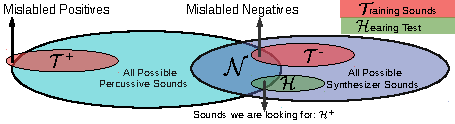
\includegraphics[width=1\linewidth]{images/chapter_4/venn_data.pdf}}
    \end{center}
    \caption{ An illustration of the discrepancy between the sounds used to train the classifiers and the type of sounds the classifier is expected to classify. $\mathcal{N}$ is the set of percussive sounds a synthesizer is capable of making. The inclusion of sounds in this group may vary from person to person. The positive samples, $\mathcal{T^{+}}$, is a small fraction of a wide variety of percussive sounds that are conceivable. For $\mathcal{T^{-}}$, Any number of random samples can be generated. $\mathcal{H}$ is a series of sounds sent to the ear for classification.}
\label{fig:ven_data}
\end{figure}
 With the datasets of labeled drum sounds, discussed in Section~\ref{sec:datasets}, we implemented several algorithms for categorizing unlabeled drum sounds, given that they are drum sounds. However, a major hurdle towards the implementation of a \enquote{drum from non-drum} recognizer is that the set of sounds that are not percussive is infinite. Drum groups are an example of closed sets, since it is reasonable that a sufficiently large sample pack can effectively describe common drum categories. However, effective representation of all possible non-drum sounds is not attainable via examples alone.

Traditional classification tasks often make the assumption the data points used for training the model and future unlabeled data will emerge from the same system of processes~\cite{geng2020recent,mundt2019open}. This assumptions requires that sufficient positive examples of all possible classes exist and are trained on. Works which involve the implementation of GANs have documented scenarios in which networks will assign high categorization probabilities to nonsensical, out of context data which should be rejected rather than categorized~\cite{geng2020recent,mundt2019open,hassen2020learning}. \\

\section{Ear Decisions}
\label{sec:decisions}
 Having considered the caveats and requirements, once a sound is generated and passed onto the ear, we expect the virtual ear to make decisions in response to two important questions: 
\emph{
\begin{quote}
\text{Decision.1 Could the sound be used as a drum?}\label{Decision.1}
\\
\text{Decision.2 If it does sound like a drum, what type of drum should it be?}\label{Decision.2}
\end{quote}
    }
\decfirst~requires knowledge of what drums \textbf{do not} sound like, or knowledge of an infinitely large set, which cannot be fully represented via examples. An important consideration is that the source of sounds used for training the model (organic drum sounds) will be fundamentally different from the source of unlabeled sounds we wish to categorize (noise from a synthesizer). This issue is reflective of the open set recognition (OSR) problem~\cite{geng2020recent,mundt2019open}. Figure~\ref{fig:ven_data} to highlights a number of caveats with our training approach. If the sound is deemed percussive, the virtual ear makes \decsecond~by finding the best drum category for the sound. The number of categories available is dependent on the database of drums used for training. 
% To maximize the transference of knowledge gained from training the classifiers to evaluation of programs, we need to extract concise feature sets that capture fundamental characteristics of the data points.

The goal is to create a pipeline of sound generation where the synthesizer is used for the rapid generation of sounds and the virtual ear is used for the acceptance of inputs which satisfy some fundamental characteristics of percussive instruments. The representation of sounds is critical in allowing the acceptance of novel sounds as part of the drum group despite their anomalies. In the previous chapter, we discussed 2 different approaches to feature extraction. This leads to two different implementation of a virtual ear: \emph{two phased ears} (TPEs) and \emph{mixed ear models} (MEMs). TPEs are a combination different models for each of \decfirst~and \decsecond. The features utilized by these models are manually defined. MEMs use a highly compressed, automatically encoded representation of sound to give simultaneous answers to both questions.


\subsection{Two Phased Ears}
\begin{figure}[t!]
    \begin{center}
    \textbf{TPE Design}
    \makebox[\textwidth]{
    \fbox{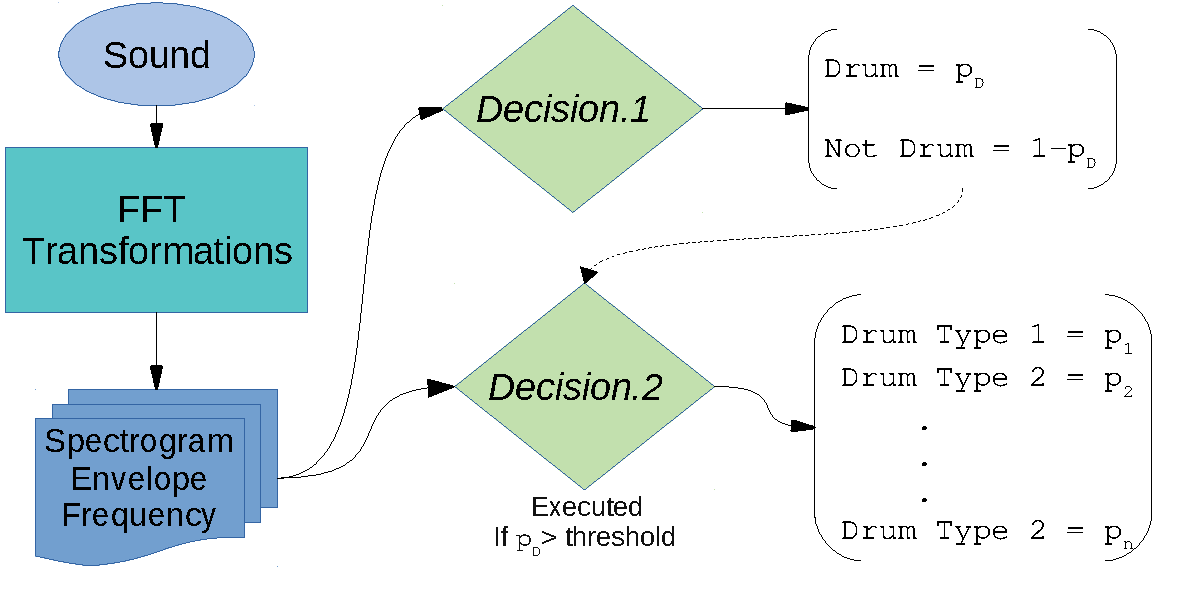
\includegraphics[width=1.1\linewidth]{images/chapter_4/TPE_ear.pdf}}}
    \end{center}
    \caption{TPE's receive a sound and make decisions sequentially.}
\label{fig:TPE_design}
\end{figure}


\label{TPE_models}
Using the features and transformation described in the previous chapter as input, we trained several neural network models with the pytorch library. The tasks at hand with regards to \decfirst~is to separate drums from not-drums (DrumVsNotDrum, or DVN). In \decsecond~the aim is to categorize the type of drums and percussion (DrumVsDrum, or DVD). 

 Multiple neural network architectures using different subsets of the FFT features to specialize in \decfirst~or \decsecond~are combined to make decisions sequentially. For \decfirst, all drums in RadarDB and FreeDB and 6000 examples of virtual synthesizer noise are used. For \decsecond, we combined the two databases and merge toms into kicks and rims/shakers into \enquote{other}. 80\% of this dataset were used for training, and the remaining 20\% of sounds for testing. 98\% accuracy in \decfirst~and 82\% accuracy in~\decsecond~were achieved with the best models. The loss function and optimizer are Categorical Cross-Entropy and Adam respectively. Training continued until no reduction in loss and accuracy is observed for 10 epochs. These accuracy numbers are weak as we did not account for category sizes or cross validate.  


\subsubsection{DVN Models}
\textbf{FC-DVN}: Fully connected network trained on Envelope features, reaching 97\% accuracy on the test data for~\decfirst. 
\begin{center}
\vbox{
    \begin{lstlisting}[caption=Sequential Layers for FC-DVN]
            Layer                       Details
            ========================================================
            Linear                      in_features=400 
                                        out_features=20 
                                        bias=True
            PReLU                       
            Linear                      in_features=20
                                        out_features=10 
                                        bias=True
            PReLU
            Linear                      in_features=10
                                        out_features=4
                                        bias=True
            PReLU
            Linear                      in_features=4
                                        out_features=2
                                        bias=True
            Softmax                     DVN probabilities
                        
        \end{lstlisting}}
\end{center}
\textbf{CNNLSTM-DVN}: A combination of CNN and LSTM models, where the CNN model extracts higher level features that are fed temporally to an LSTM cell. This model is trained on spectrum data and reaches 98\% accuracy on the test set. 
\begin{center}
\vbox{
    \begin{lstlisting}[caption=Sequential Layers for CNNLSTM-DVN]
            Layer                       Details
            ========================================================
            Conv2d                  kernel size = (7, 3)
                                    stride = (1, 1)
                                    padding = (3, 1)
            ReLU
            Dropout                 probability = 0.5
            LSTMCell                hidden size = 800
                                    input size = @($\mathcal{F}$)@
            Linear                  in_features = @($\mathcal{F}$)@
                                    out_features = 2
                                    bias=True
            Softmax                 DVN probabilities
\end{lstlisting}}
\end{center}

\subsubsection{DVD Models}
\textbf{E+F-DVD}: A fully connected model trained on a concatenation of envelope and frequency features. Reaching 80\% accuracy for 6-way drum categorization in Phase 2. 
\begin{center}
\vbox{
    \begin{lstlisting}[caption=Sequential Layers for E+F-DVD]
            Layer                       Details
            ========================================================
            Linear                      in_features = 10+50 
                                        out_features = 30
                                        bias = True
            PReLU                       
            Linear                      in_features = 30
                                        out_features = 10
                                        bias = True
            PReLU                       
            Linear                      in_features = 10
                                        out_features = 10
                                        bias = True
            PReLU     
            Linear                      in_features = 10
                                        out_features = @($\mathcal{C}$)@
                                        bias = True
            Softmax                     drum type probabilities
        \end{lstlisting}}
\end{center}

\textbf{CNN-DVD}: A CNN model trained on Spectrum features. Reaching 82\% accuracy in a 6-way drum categorization in Phase 2.  
%  {\color{red}double check architecture}
\begin{center}
\vbox{
    \begin{lstlisting}[caption=Sequential Layers for CNNLSTM-DVD]
            Layer                       Details
            ========================================================
            Conv2d                  kernel size = (7, 3)
                                    stride = (1, 1)
                                    padding = (3, 1)
            ReLU
            Dropout                 probability = 0.5
            LSTMCell                hidden size = 800
                                    input size = @($\mathcal{F}$)@
            Linear                  in_features = @($\mathcal{F}$)@
                                    out_features = 2
                                    bias=True
            Softmax                 DVD probabilities
\end{lstlisting}}
\end{center}

\textbf{FC-DVD}: Fully connected 3 layer neural net with 78\% accuracy for 6-way drum categorization in Phase 2. 
\begin{center}
\vbox{
    \begin{lstlisting}[caption=Sequential Layers for FC-DVD]]
            Layer                       Details
            ========================================================
            Linear                      in_features=400
                                        out_features=20 
                                        bias=True
            PReLU                       
            Linear                      in_features=20
                                        out_features=10 
                                        bias=True
            PReLU
            Linear                      in_features=10
                                        out_features=4
                                        bias=True
            PReLU
            Linear                      in_features=4
                                        out_features=@($\mathcal{C}$)@
                                        bias=True
            Softmax                     drum type probabilities
                        
        \end{lstlisting}}
\end{center}
\subsubsection{Finalzing TPEs}
These models can be combined and weighted in various ways and the confidence thresholds can be modified in order to implement \enquote{virtual ears} with different properties. A glaring issue in the current implementation is the treatment of softmax outputs as a reasonable measure of a model's confidence. As a result, some models may have unwarranted higher confidence in their scores, skewing attempts at finding a consensus.  

With the models showing high accuracy on testing data, they can be combined in order to make decisions sequentially. For \decfirst~we only determine sounds as percussive if both FC-DVN and CNN-LSTM have categorized it as such with over 90\% confidence. For the majority of random generations, that is not the case, but if a randomly generated sound has passed this phase, the three categorizers assign their categorizations to this sound.  These categorizers have a moderate degree of agree-ability as seen in Section~\ref{surveys}, but often the decision is not unanimous.

% The fourth method of categorization, \enquote{averaged-cat}, is implemented by taking the sum of the softmax outputs of all three categorizers, using it to determine the category.



\subsection{Mixed Ear Models}

\begin{figure}[t!]
    \begin{center}
    \textbf{MEM Design}
    \makebox[\textwidth]{
    \fbox{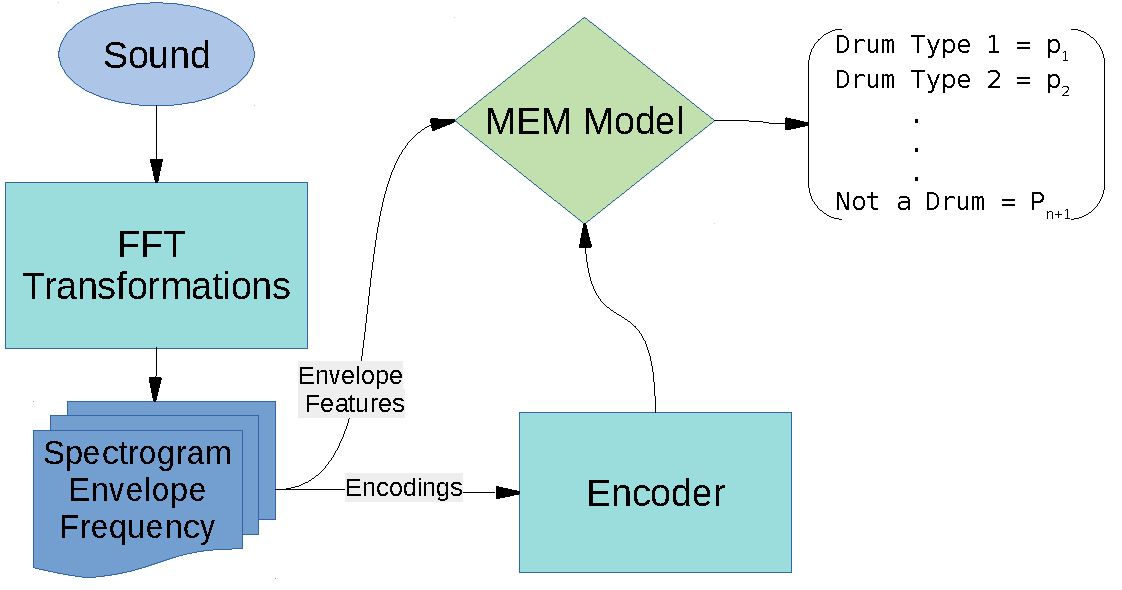
\includegraphics[width=1.1\linewidth]{images/chapter_4/MEM_ear.pdf}}}
    \end{center}
    \caption{MEMs use both FFT features and embedding features to make both decisions simultaneously. }
\label{fig:TPE_design}
\end{figure}
\label{chap3:mixed_ear_models}
In Section~\ref{section:embedded_feats}, the potential use for embedded features in categorization was visualized using t-SNE. As t-SNE results are not classifiers in of themselves, there is a need for a model which uses encodings of each sound group to predict its type. This differs from two-phased ears as the model is simultaneously categorizing a new sound's drum type or putting it in the \enquote{synthetic noise} category. We call this task drum vs drum vs not-drum, or \enquote{DvDvN}. We also tackle \decfirst~using embedded features, although DvN MEM models are not used in the final pipelines.

As mentioned previously, manual t-SNE inspections highlighted a disregard for envelope shapes as a major source of failure. The performance of the models before and after the addition of envelope features (a vector of size 10) to the feature space is shown in Figures~\ref{fig:f1_allg_box} and ~\ref{fig:f1_dvn_box}. 

The autoencoder model trained on MixedDB is used as an embedding feature extractor. RadarDB, FreeDB and NoiseDB are combined for training/test data. To prevent class overlaps as much as possible, claps, hats, kicks, snares and synthetic noise groups are used for measuring model effectiveness. Samples longer than 1 second are excluded, to reduce potentially mislabeled data. Final training database for mixed ear models is described in Table~\ref{db:memDB}.
\begin{table}[htbp]
\centering
\begin{tabular}{|l|l|l|l|l|l|}
\hline
 DB Name & kick & snare & clap & hat & Synthetic Noise\\\hline
 MixedEarDB & 1334 & 1035 & 401 & 1275 & 1000 \\ \hline
\end{tabular}
\caption{MixedEarDB: A database put together by combination of radarDB, FreeDB and NoiseDB}
\label{db:memDB}
\end{table}

\subsubsection{Model Selection}
Using embeddings and envelope features to represent audio, five classification models were trained for the task of categorizing the five different sound groups. For hyper-parameter optimization, the models were trained using 5-fold cross validation and 80/20 train-to-test ratio. The F-Score result of each cross-validation is the unweighted average F-Score of all groups. For inter-model comparisons, the procedure is the same except 10-fold cross validations are used. The models were derived from scikit-learn's implementations of these classifiers~\cite{pedregosa2011scikit}. Before inter-model comparisons, we conducted a grid-search for each model on at least one of its possibly decisive hyper-parameters. The classifiers and other notable specifications are presented in Table~\ref{table:mem_model_selection}. Class weights were used where possible to mitigate the effects of an imbalanced dataset~\cite{provost2000machine,chawla2004special}. When utilized, the weight for each class $c$ is calculated as:

\begin{subequations}
    \begin{align*}
    c_{weight} = 1-\dfrac{\text{Number of samples in group $c$} }{\text{Total number of samples}}
    \end{align*}
\end{subequations}

\begin{table}[t]
    \centering \hspace*{-0.8cm}
    \begin{threeparttable}
    \begin{tabular}[width=0.95\paperwidth]{|l|l|l|}
    \hline
    Model name & Tuned Parameters\tnote{\dag}  & Used Weights? \tnote{\ddag} \\\hline
     Support Vector Classifier (SVC) &  Gamma:0.001, C:100, kernel:rbf & Yes\\
     LinearSVC & C:10 & Yes\\
     K Nearest Neighbors & Num. Neighbors:31 &  No \\
     Random Forest Classifier & Num Estimators:500 & Yes \\
     Extra Trees Classifier & Num Estimators:1100 & Yes\\
     \hline
    \end{tabular}
    \caption{Models implemented for comparison using envelope and embedded features. }
    \begin{tablenotes}
    \item[\dag] Tuned parameters values are based on grid-searching for best f-score. Parameters not mentioned have neither been tuned nor changed from scikit-learn's default values (as of version 0.23)
    \item[\ddag] Class weights are used unless not applicable to classifier.
    \end{tablenotes}
    \label{table:mem_model_selection}
    \end{threeparttable}
\end{table}

\begin{figure}[htbp!]
    \begin{center}
    \textbf{Cross Validation F-Scores For All Sound Groups}\par\medskip
    \makebox[\textwidth]{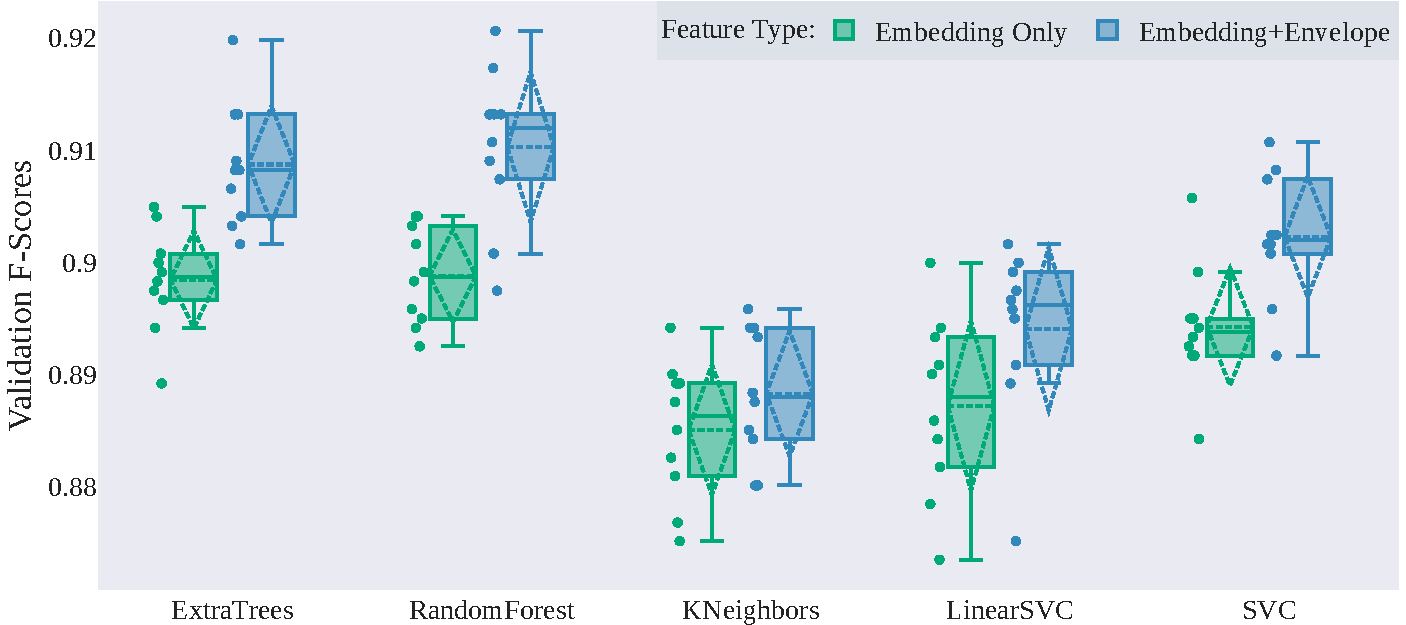
\includegraphics[width=0.8\paperwidth]{images/chapter_3/mme_comparisons_mme.pdf}}
    \caption{Boxplots visualizing the F-Score results for each cross-validation. The individual scores, means, medians, standard-deviation and outliers are depicted. The differences are noticeable, yet means lie within the \%88-92 range. Envelope features improve classification accuracy for all models. }
    \label{fig:f1_allg_box}
    \end{center}
\end{figure}

We're also interested in how these models perform on the binary DvN task (i.e \decfirst).
After grouping all drums together, the model selection is repeated. A repeat the hyper-parameter optimization step did not highlight any necessary changes except for a reduction in the number of neighbors for the K-Neighbor model (from 30 to 5). As shown in in Figures~\ref{fig:f1_allg_box} and~\ref{fig:f1_dvn_box}, the addition of envelope features had a positive effect on performance for all mdoels, yet the RandomForest and ExtraTrees models clearly outperform the other classifiers in both tasks. We train the top models on \%80 of the database and use the remaining \%20 to create the confusion matrices and the F-Scores shown in Figure~\ref{fig:conf_f1_dvn}.
\begin{figure}[h!]   
    \begin{center}
        \textbf{Cross Validation F-Scores For Drum Vs Not-Drum}
    \makebox[\textwidth]{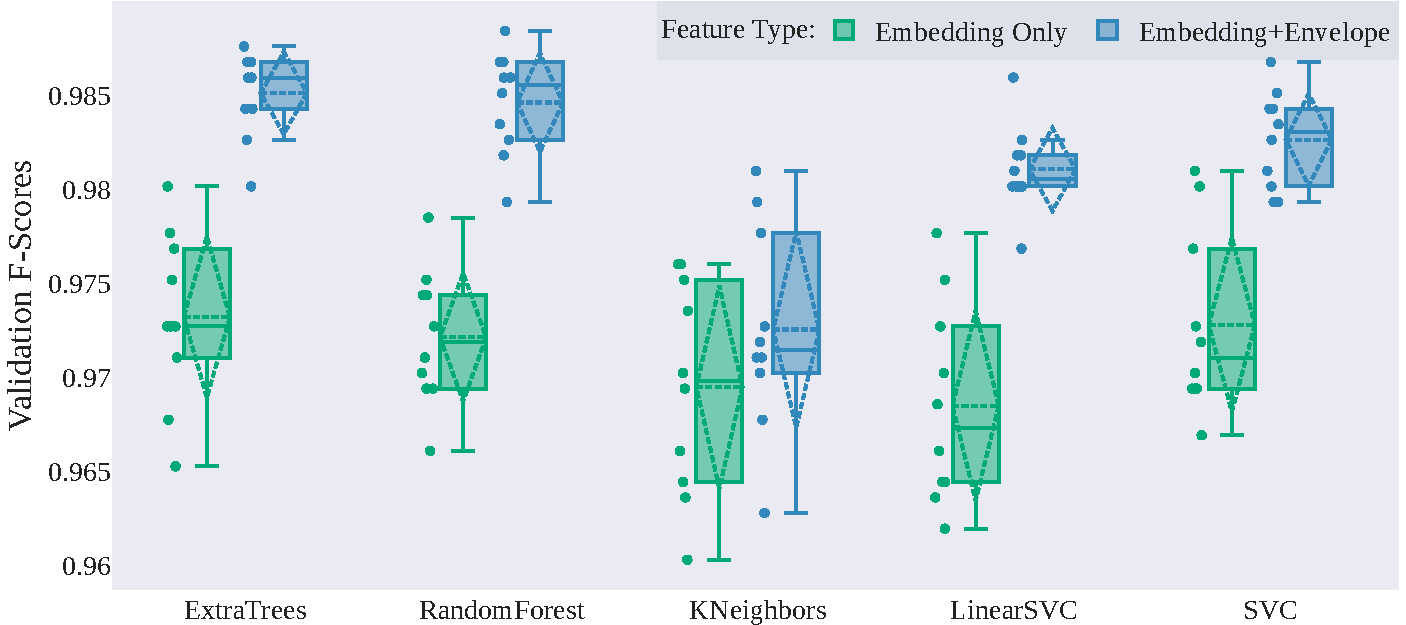
\includegraphics[width=0.8\paperwidth]{images/chapter_3/mme_comparisons_dvn.pdf}}
    \caption{F-Score results for each cross-validation. Models perform better as there are less categorization groups. Envelope features increase accuracy for all models. Random Forest and Extra Trees remain the top two models. }
    \label{fig:f1_dvn_box}
    \end{center}
\end{figure}


\begin{figure}[htbp!]
\begin{center}
    \textbf{ Classification Report for DvDvN and DvN  }\par\medskip
    \makebox[\textwidth]{
    \subfloat[Precision, recall, F1-Score, and number of supporting examples]{ 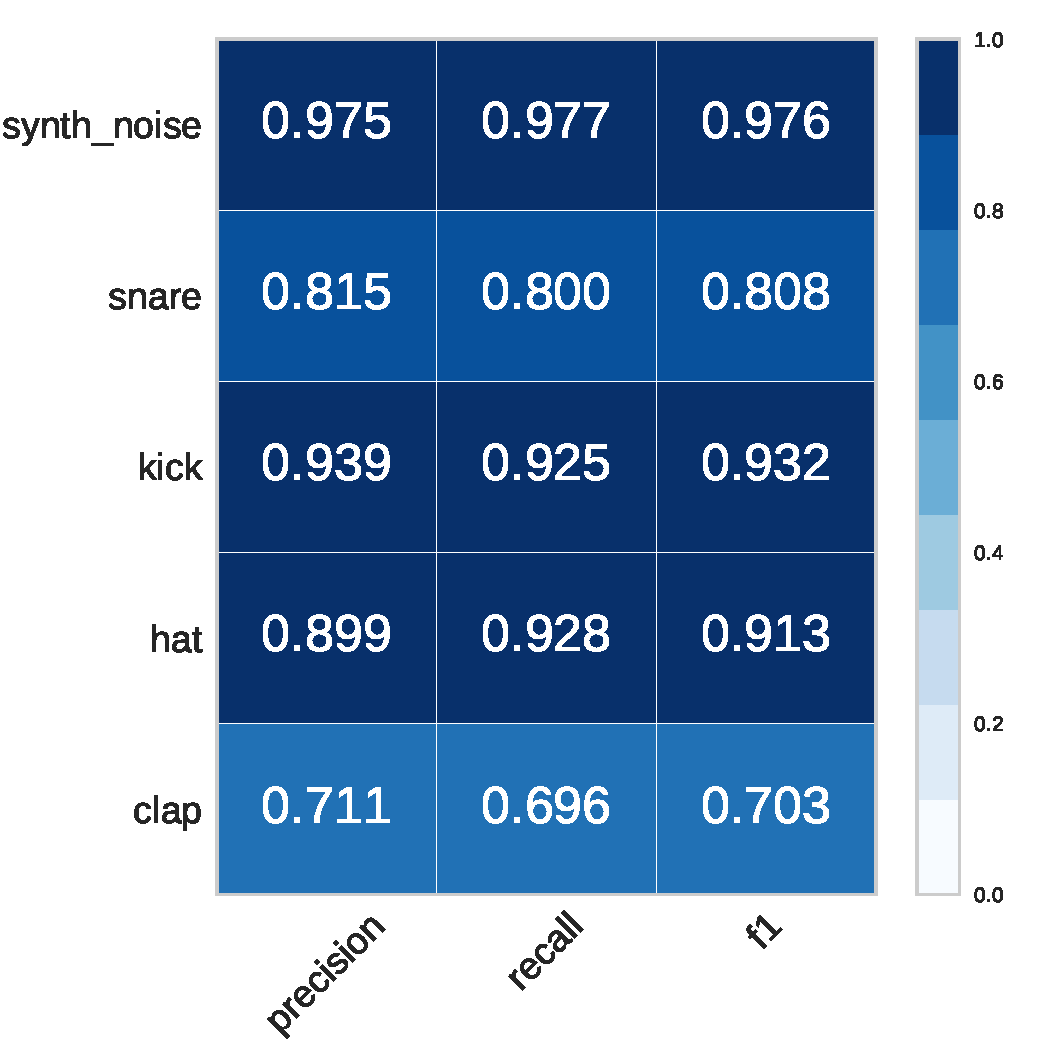
\includegraphics[width=9cm,height=9cm]{images/chapter_3/f1_mme.pdf}
    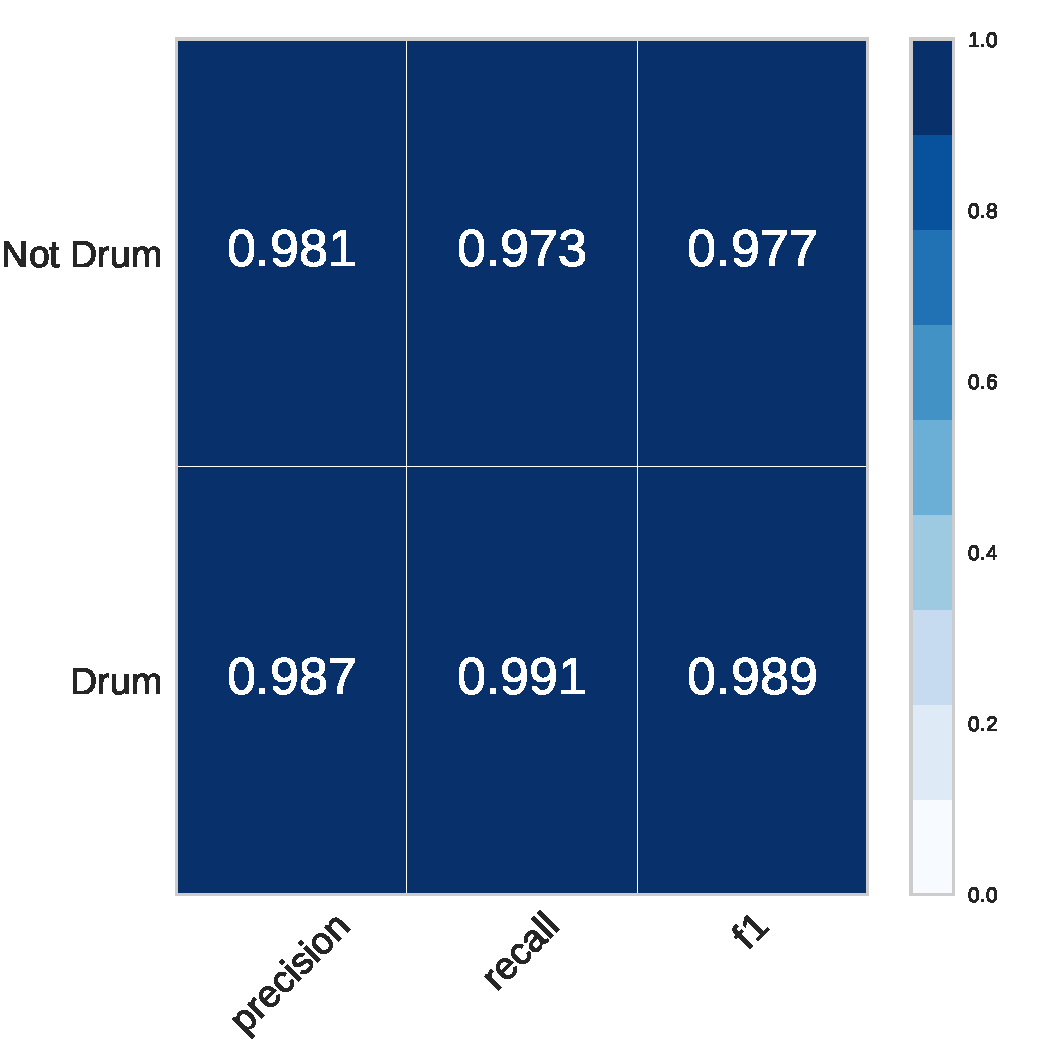
\includegraphics[width=9cm,height=9cm]{images/chapter_3/f1_dvn.pdf}
    }
    
    }
\label{fig:conf_f1_dvd}
\end{center}

\begin{center}
    \makebox[\textwidth]{
    \subfloat[Confusion matrices]{ 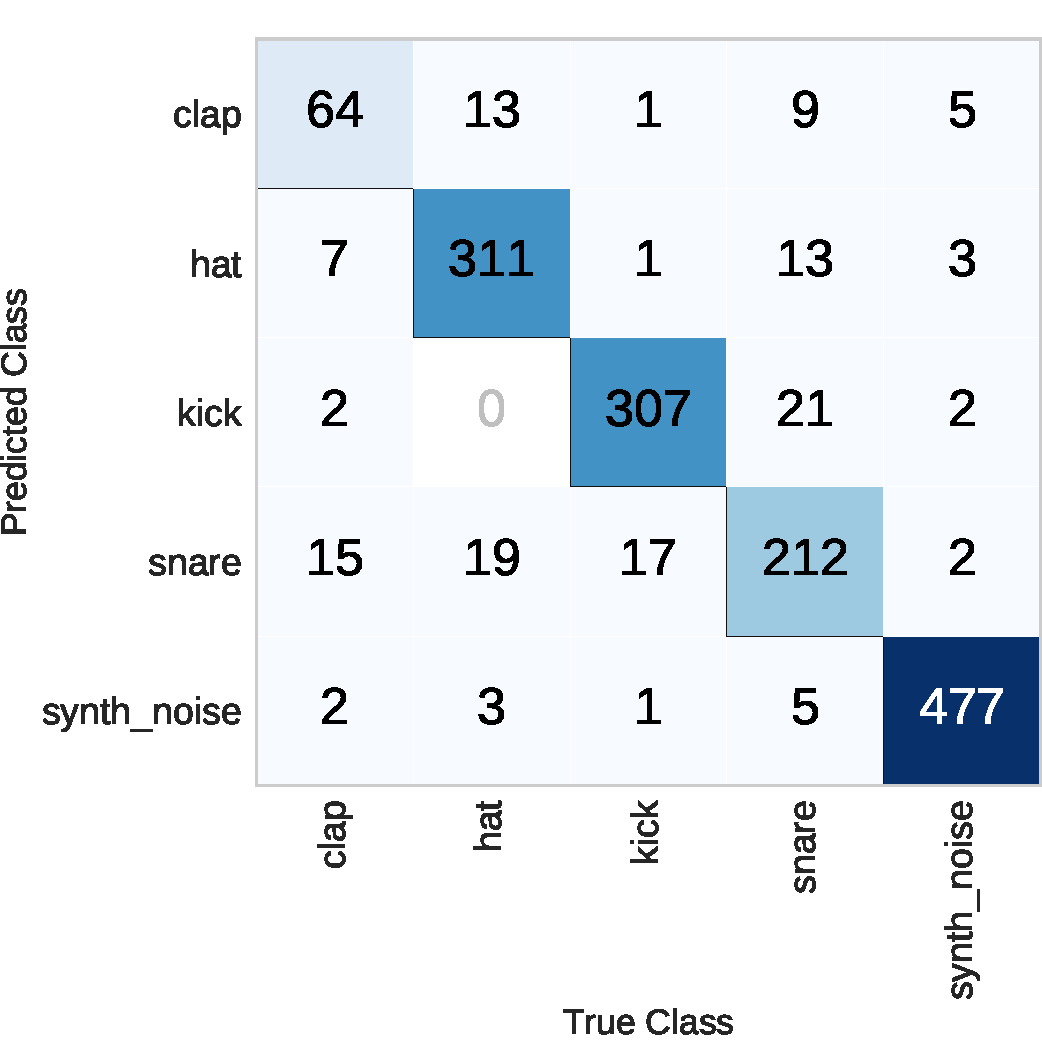
\includegraphics[width=9cm,height=9cm]{images/chapter_3/conf_mme.pdf}
    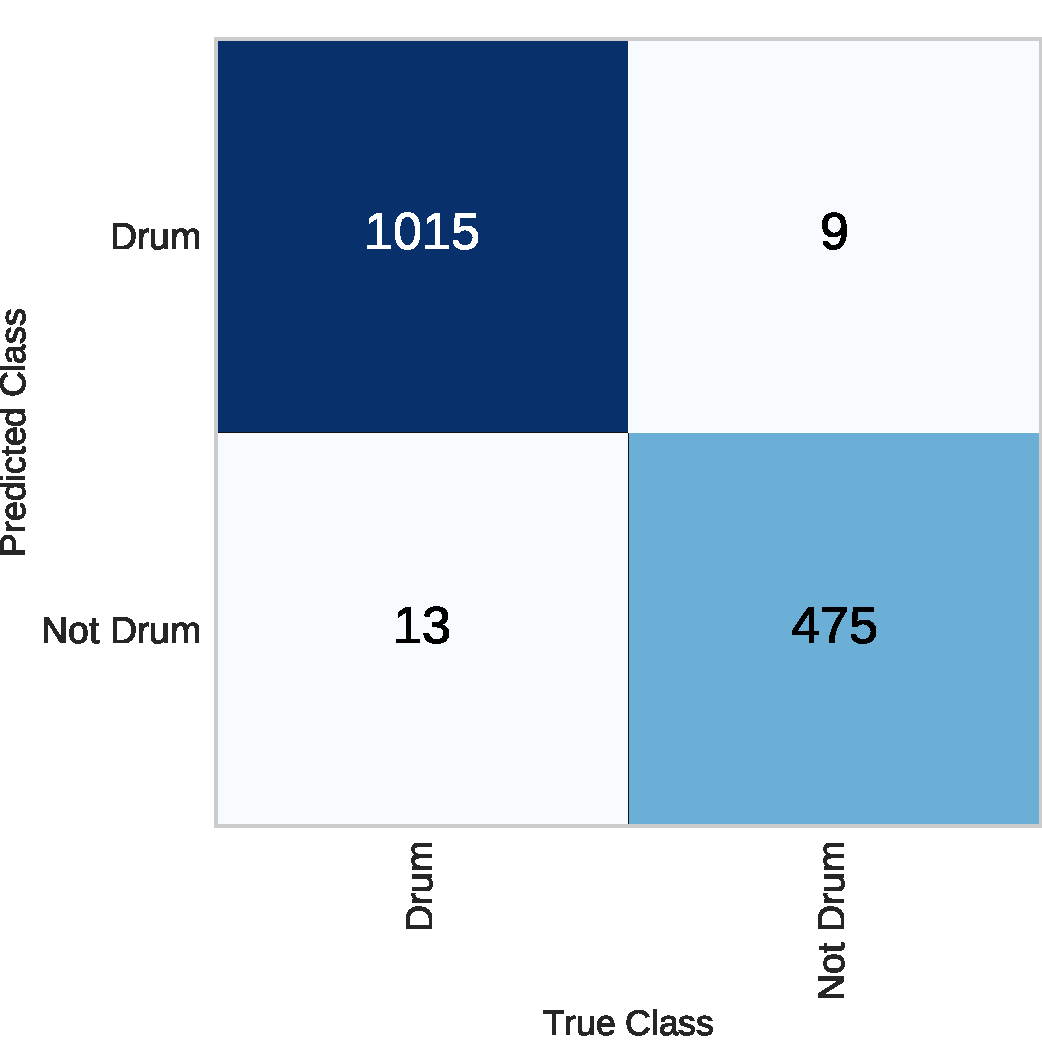
\includegraphics[width=9cm,height=9cm]{images/chapter_3/conf_dvn.pdf}
    }}
\end{center}


\caption{F-Scores and confusion matrix of ExtraTrees model for both DvDvN and DvN categorization.}
\label{fig:conf_f1_dvn}
\end{figure}

Based on these reports, having multiple options for drum categorization does not noticeably influence the models accuracy in \decfirst. However, the DvDvN models' slightly smaller false negative rate for synthetic noise (11 vs 13 false negatives) is countered by a slightly higher rate of categorizing drums as synthetic noise (12 vs 9). Therefore, the DvDvN implementation is used as it makes the DvN model redundant.

The finalized MEM is created by combining the encoder with the ExtraTrees classifier. As sounds are generated with the virtual synthesizer, the encoding and envelope features will be extracted using the encoder and sent to the ExtraTrees DvDvN classifier. In the upcoming \enquote{Novel Generations} Chapter, we will present the results of a two person survey where the accuracy of the different models is analyzed given over 500 synthetic noise sounds categorized as drums. 




% \section{Is the Virtual Synthesizer Deterministic?}
% \label{section:synth_deterministic}
% It is crucial that rendering the audio from the same synthesizer program results in identical, or near identical sounds. Our synthesizer modules are capable of producing random waves, or \enquote{noise}. This type of sound will vary each time it is produced. Manual listening does not show sonic variation between multiple creation of the same set of parameters, but how does this affect the ear models?

% We create 50 parameter sets for stack sizes of 1 and evaluate each parameter set 10 times using the CNN-DVN model. This model outputs the probability of a sound belonging to the drum/percussion category (Discussed previously in Section~\ref{TPE_models}). Put simply, we are creating the sonic output given the same program multiple times and recording the predicted value from the model. We repeat this experiment for stack sizes of 2 and 8 and show the results in Figure~\ref{fig:synth_deterministic}. 

% \begin{figure}[htbp!]
% \begin{center}
%     \textbf{ Variation in Repeated Evaluations of Synthesizer Programs }\par\medskip
%     \makebox[\textwidth]{
%     \subfloat[1 Stack]{ 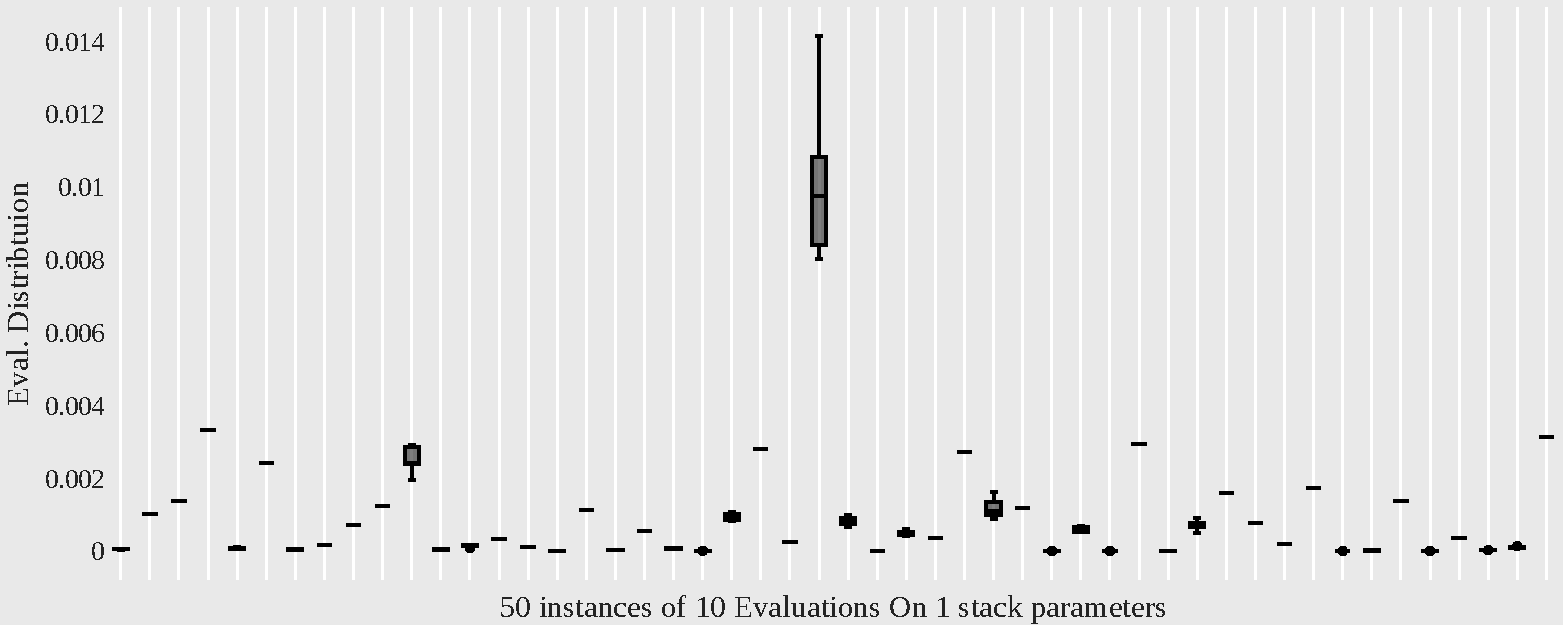
\includegraphics[width=17cm,height=5.67cm]{images/chapter_3/eval_stability_stacksize1.pdf}

%     }}

%     \makebox[\textwidth]{
%     \subfloat[2 Stacks]{ 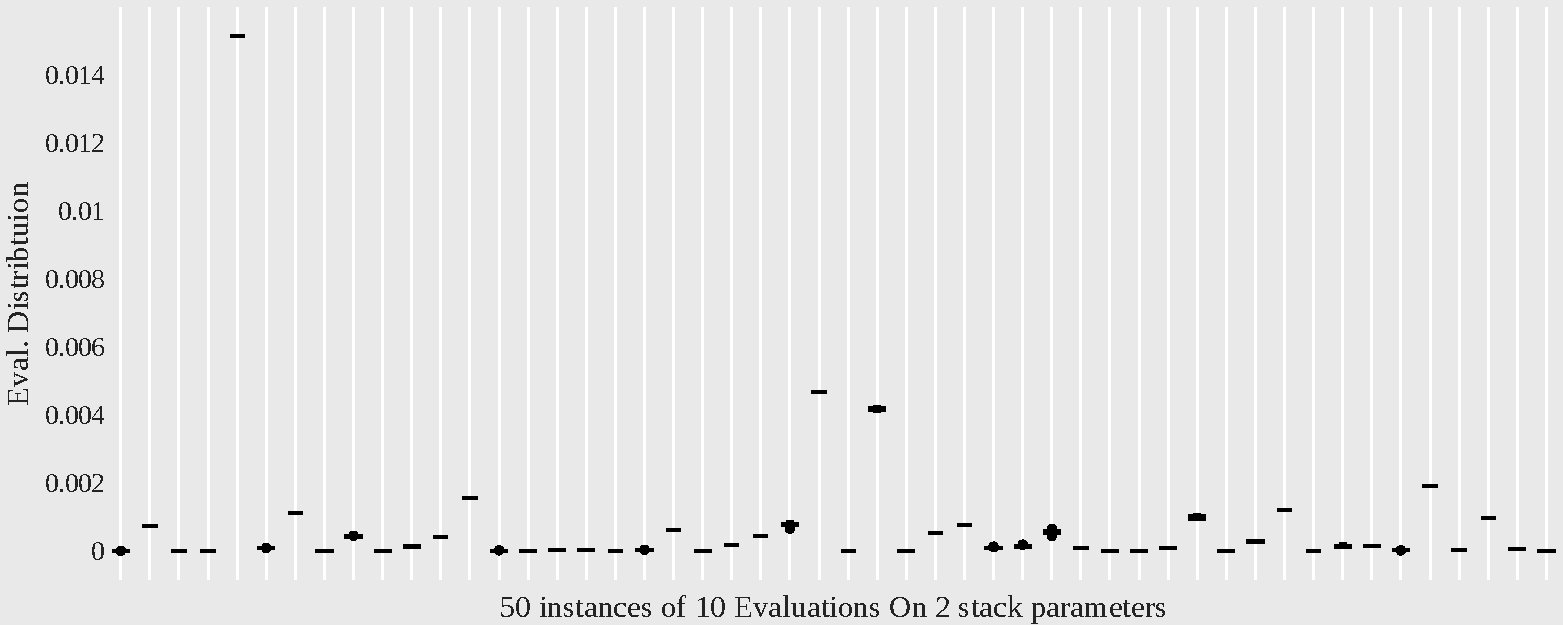
\includegraphics[width=17cm,height=5.67cm]{images/chapter_3/eval_stability_stacksize2.pdf}

%     }}
    
%     \makebox[\textwidth]{
%     \subfloat[8 Stacks]{ 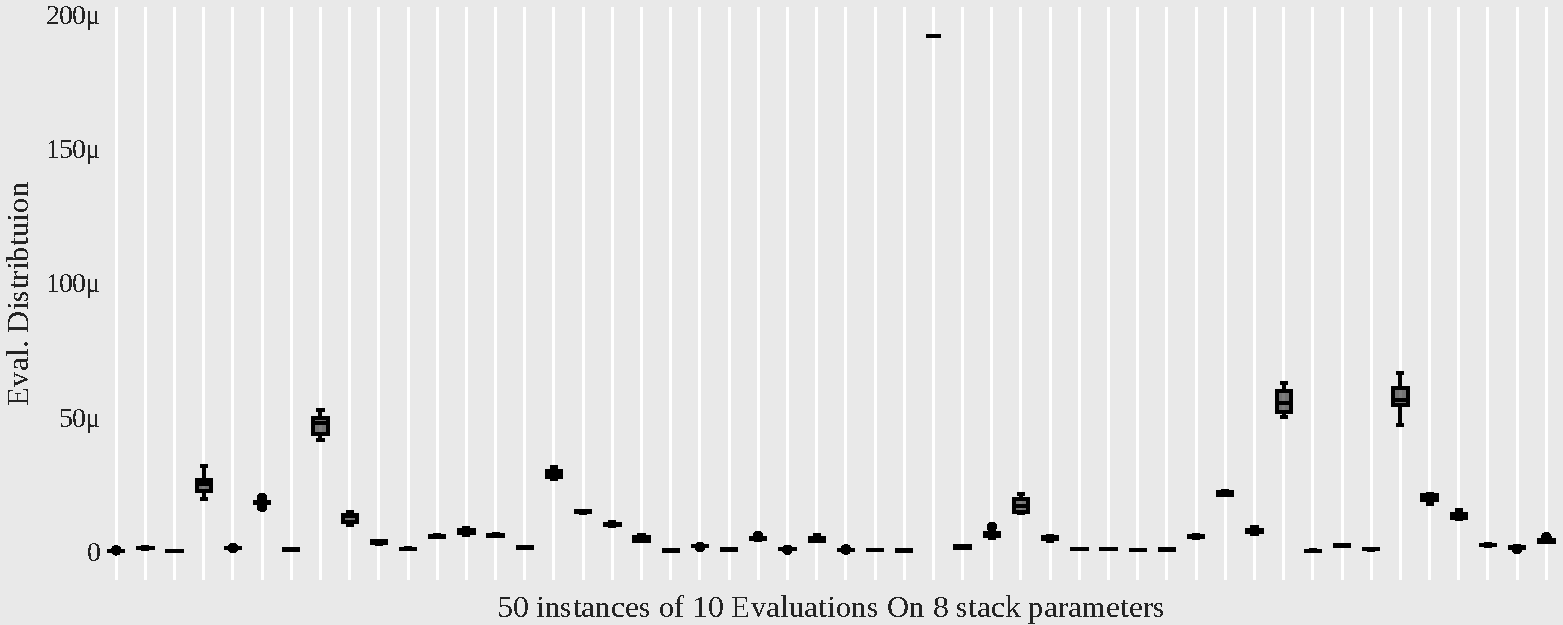
\includegraphics[width=17cm,height=5.67cm]{images/chapter_3/eval_stability_stacksize8.pdf}

%     }}
% \end{center}

% \caption{Repeated evaluation of signals from identical paramter-sets shows little variation in scores. Multiple renditions of the same parameter-set vary if the parameter-set calls for generation of 1 or more random wave-shapes..}
% \label{fig:synth_deterministic}
% \end{figure}
\end{document}